\section{eo\-Time\-Varying\-Loop\-Eval$<$ EOT $>$ Class Template Reference}
\label{classeo_time_varying_loop_eval}\index{eoTimeVaryingLoopEval@{eoTimeVaryingLoopEval}}
{\bf eo\-Pop\-Loop\-Eval}{\rm (p.\,\pageref{classeo_pop_loop_eval})}: an instance of {\bf eo\-Pop\-Eval\-Func}{\rm (p.\,\pageref{classeo_pop_eval_func})} that simply applies a private {\bf eo\-Eval\-Func}{\rm (p.\,\pageref{classeo_eval_func})} to all offspring AND ALL PARENTS as the fitness is supposed here to vary  


{\tt \#include $<$eo\-Pop\-Eval\-Func.h$>$}

Inheritance diagram for eo\-Time\-Varying\-Loop\-Eval$<$ EOT $>$::\begin{figure}[H]
\begin{center}
\leavevmode
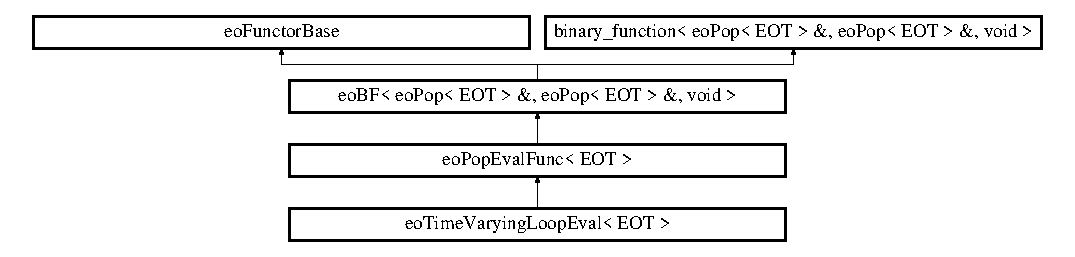
\includegraphics[height=3.01075cm]{classeo_time_varying_loop_eval}
\end{center}
\end{figure}
\subsection*{Public Member Functions}
\begin{CompactItemize}
\item 
{\bf eo\-Time\-Varying\-Loop\-Eval} ({\bf eo\-Eval\-Func}$<$ {\bf EOT} $>$ \&\_\-eval)\label{classeo_time_varying_loop_eval_a0}

\begin{CompactList}\small\item\em Ctor: set value of embedded {\bf eo\-Eval\-Func}{\rm (p.\,\pageref{classeo_eval_func})}. \item\end{CompactList}\item 
void {\bf operator()} ({\bf eo\-Pop}$<$ {\bf EOT} $>$ \&\_\-parents, {\bf eo\-Pop}$<$ {\bf EOT} $>$ \&\_\-offspring)\label{classeo_time_varying_loop_eval_a1}

\begin{CompactList}\small\item\em Do the job: simple loop over the offspring. \item\end{CompactList}\end{CompactItemize}
\subsection*{Private Attributes}
\begin{CompactItemize}
\item 
{\bf eo\-Eval\-Func}$<$ {\bf EOT} $>$ \& {\bf eval}\label{classeo_time_varying_loop_eval_r0}

\end{CompactItemize}


\subsection{Detailed Description}
\subsubsection*{template$<$class EOT$>$ class eo\-Time\-Varying\-Loop\-Eval$<$ EOT $>$}

{\bf eo\-Pop\-Loop\-Eval}{\rm (p.\,\pageref{classeo_pop_loop_eval})}: an instance of {\bf eo\-Pop\-Eval\-Func}{\rm (p.\,\pageref{classeo_pop_eval_func})} that simply applies a private {\bf eo\-Eval\-Func}{\rm (p.\,\pageref{classeo_eval_func})} to all offspring AND ALL PARENTS as the fitness is supposed here to vary 



Definition at line 84 of file eo\-Pop\-Eval\-Func.h.

The documentation for this class was generated from the following file:\begin{CompactItemize}
\item 
eo\-Pop\-Eval\-Func.h\end{CompactItemize}
